\documentclass{beamer}
\title{Git Basics}
\author{David Kouka}
\date{\today}

\usepackage{graphicx}   % For including images
\usepackage{listings}   % For code listings
\usepackage{tikz}       % For diagrams
\usetikzlibrary{arrows.meta, positioning, shapes.geometric}

\lstset{
    basicstyle=\ttfamily\color{blue}, % Change color and font
    keywordstyle=\color{red},
    commentstyle=\color{green},
    stringstyle=\color{orange},
    columns=flexible,
    keepspaces=true,
    showstringspaces=false,
}

\begin{document}

\frame{\titlepage}  % Title slide

\section{Table of Contents}

\begin{frame}
\tableofcontents
    \begin{center}
        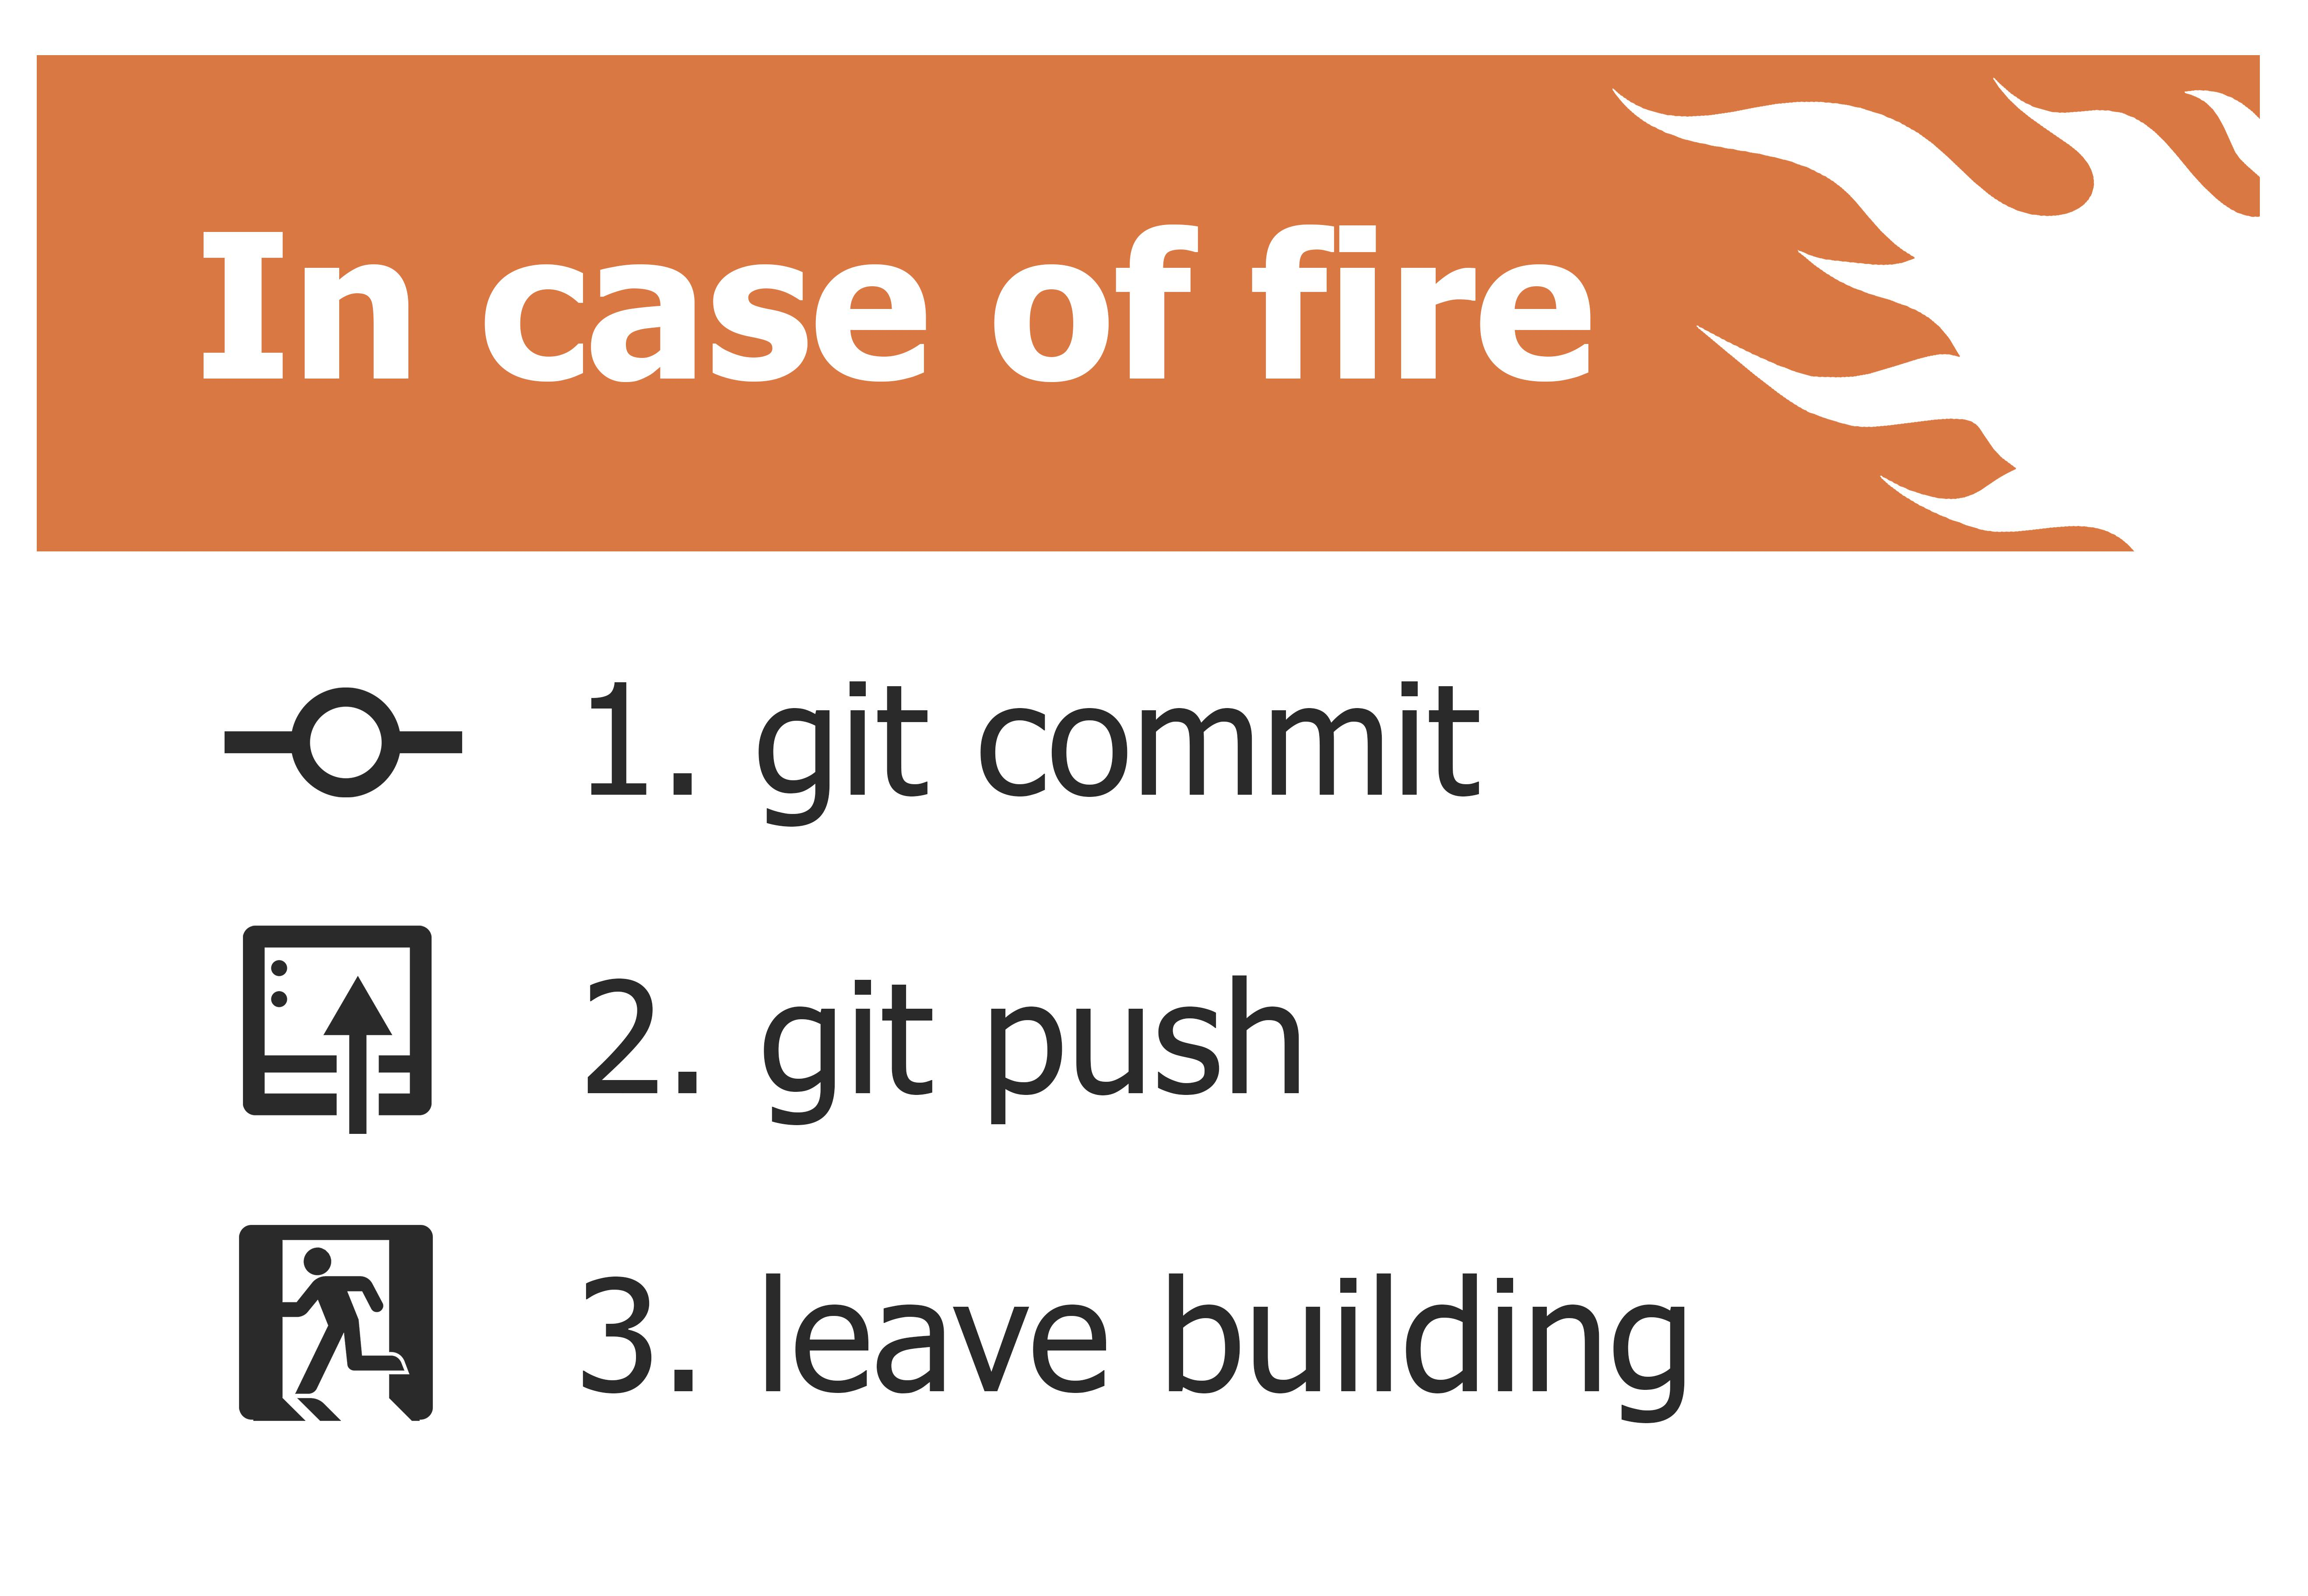
\includegraphics[width=0.5\linewidth]{img/in_case_of_fire.jpg}
    \end{center}
%TODO
\end{frame}

\section{Version control}


\begin{frame}{Illustrating Git Branches and Commits}
    \begin{center}
        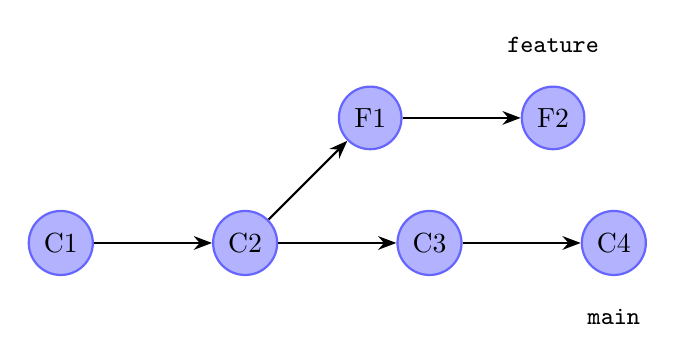
\begin{tikzpicture}[
            commit/.style={circle, draw=blue!60, fill=blue!30, thick, minimum size=6mm},
            branch/.style={draw, thick, -{Stealth}},
            label/.style={font=\small\ttfamily},
            node distance=1.5cm
        ]

            % Main branch
            \node[commit] (c1) {C1};
            \node[commit, right=of c1] (c2) {C2};
            \node[commit, right=of c2] (c3) {C3};
            \node[commit, right=of c3] (c4) {C4};
            
            % Feature branch
            \node[commit, above right=1cm and 1cm of c2] (f1) {F1};
            \node[commit, right=of f1] (f2) {F2};
            
            % Arrows for main branch
            \draw[branch] (c1) -- (c2) node[midway, above] {};
            \draw[branch] (c2) -- (c3) node[midway, above] {};
            \draw[branch] (c3) -- (c4) node[midway, above] {};

            % Arrows for feature branch
            \draw[branch] (c2) -- (f1) node[midway, above] {};
            \draw[branch] (f1) -- (f2) node[midway, above] {};
            
            % Branch labels
            \node[label, below=0.3cm of c4] {main};
            \node[label, above=0.3cm of f2] {feature};
            
        \end{tikzpicture}
    \end{center}
\end{frame}

\begin{frame}{Why using version control}
    \begin{itemize}
        \item<1-> Tracking changes \lstinline{git diff}
        \item<2-> Backup and recovery \lstinline{git checkout}
        \item<3-> Collaborative work (authors, conflicts, PR)
        \item<4-> Accountability \lstinline{git blame}
        \item<5-> "Documentation" via commit messages \lstinline{git log}
        \item<6-> Safe experiments \lstinline{git branch}
        \item<7-> Easy release management (tags, banches, CI/CD, ...)
    \end{itemize}
\end{frame}

\section{Git commands}

\subsection{Cloning}

\begin{frame}{git clone}
    \only<1-> Copy repository from server \pause

    \begin{itemize}
        \item<2-> Bitbucket 
        \item<3-> Gitea
        \item<4-> Github
        \item<5-> Gitlab
    \end{itemize}
\end{frame}

\begin{frame}{Illustrating Git Clone Operation}
    \begin{center}
        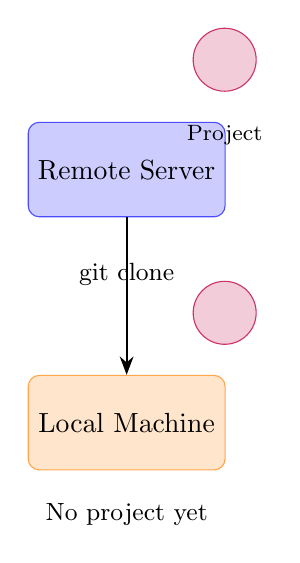
\begin{tikzpicture}[
            server/.style={rectangle, draw=blue!70, fill=blue!20, rounded corners, minimum width=2.5cm, minimum height=1.2cm},
            pc/.style={rectangle, draw=orange!70, fill=orange!20, rounded corners, minimum width=2.5cm, minimum height=1.2cm},
            project/.style={circle, draw=purple!80, fill=purple!20, minimum size=0.8cm},
            arrow/.style={thick, ->, >=Stealth}
        ]
        
            % Step 1: Initial state with remote server holding the project, and empty local machine
            \onslide<1->{
                \node[server] (remote) {Remote Server};
                \node[project, above right=0.5cm and -0.3cm of remote] (remote_project) {};
                \node[below=0.3cm of remote_project, font=\footnotesize] {Project};
            }
            \onslide<1->{
                \node[pc, below=2cm of remote] (local) {Local Machine};
                \node[below=0.3cm of local, font=\small] {No project yet};
            }

            % Step 2: Show git clone command as a label on the arrow
            \onslide<2->{
                \draw[arrow] (remote) -- node[midway, above, font=\small] {git clone} (local);
            }

            % Step 3: Local machine now has the project as well
            \onslide<3->{
                \node[project, above right=0.5cm and -0.3cm of local] (local_project) {};
            }
        
        \end{tikzpicture}
    \end{center}
\end{frame}

\end{document}

